
%\hyperlink { label } { link caption }
% \hypertarget { label } { target caption }
\documentclass{article}
\usepackage[brazil]{babel}
\usepackage[utf8]{inputenc}
\usepackage{xcolor}
\definecolor{verde}{rgb}{0,0.5,0}
\usepackage{listings}
\usepackage{hyperref}
\usepackage{graphicx}
\lstset{
  language=C++,
  basicstyle=\ttfamily\small, 
  keywordstyle=\color{blue}, 
  stringstyle=\color{verde}, 
  commentstyle=\color{red}, 
  extendedchars=true, 
  showspaces=false, 
  showstringspaces=false, 
  numberstyle=\tiny,
  breaklines=true, 
  backgroundcolor=\color{green!10},
  breakautoindent=true, 
  captionpos=b,
  xleftmargin=0pt,
}
\pagestyle{empty}


%Conteudo

  
\title{Documentação Técnica e Funcional do Software de Gerenciamento de Hotel}
\date{11 de Dezembro de 2017}
\author{João Paulo de Souza \and Marco Túlio Nogueira Cambraia}

  \begin{document}
  \maketitle
  \newpage
  \tableofcontents %%Sumário
  \newpage

  \section{Estruturação das Interna Pastas}
  	Os arquivos são estruturados na pasta interna software de forma que seguem a seguinte ordenação e nomeclatura:\\
  	\subsection{Pasta 'libs'} Guarda os arquivos com extensão .h, que são utéis no funcionamento do software. A funcionalidade específica ou fluxo de dados será explicada mais a frente.\\
  	Segue a lista dos arquivos de cabeçalho presentes na pasta citada: \\
  	\begin{enumerate}
  		\item \textbf{structs.h:} O arquivo de cabeçalho structs.h, trata somente de organizar as estruturas ou 'structs' presentes e necessárias no código fonte.;\\
  		\item \textbf{cadastros.h:} O arquivo de cabeçalho cadastros.h, trata de utilizar as estruturas, citadas no item acima, para armazenar os dados digitados pelo usuário em certas ocasiões do funcionamento do software e realizar algumas pequenas validações básicas utéis no código, como por exemplo, verificar o que o usuário deseja entre duas opções. Tudo isso irá armazenar dados que serão necessários em outros arquivos de cabeçalho que irão ser citados a frente.\\
  		\item \textbf{salvar.h:} Este arquivo de cabeçalho serve para de que depois que os dados que os dados forem armazenados pela junção dos dois arquivos citados acima, que as informações sejam reunidas e salvas em um arquivo no formato texto(txt) ou em formato binário. Neste arquivo de cabeçalho, são salvos os dados são salvos alguns dados espéficos, ou dados mais comuns, que são os dados que envolvem diretamente atividades comuns de um sistema, exemplo salvar um hospede cadastrado. Estruturas mais complexas, tem seus próprios arquivos de cabeçalho para gerenciar seus dados.\\
  		\item \textbf{consulta.h:} Este arquivo header(cabeçalho), serve para realizar alguns tipos de consultas nos arquivos que são salvos pelo software. Exemplo de umas das funcionalidades é gerar códigos auto-incrementados(códigos somados de forma automática) para o uso das structs. Outro exemplo seria a consulta de dados de structs simples, como hospede e/ou produto. E por fim mais uma de suas funcionalidades, funções de validação e de pesquisa por certos campos, exemplo, código do hospede de acordo com seu CPF.\\
  		\item \textbf{edicao.h:} Este arquivo header serve novamente para structs simples do software, como produtos e/ou fornecedores. Nela estão contidas funções para editar dados dos arquivos pertencentes as essas structs citadas anteriormente. Nessas funções é possível selecionar o que será editado, mas a preço de editar um campo por vez.\\
  		\item \textbf{exclusao.h:} Neste arquivo header, estão contidas as funções de exclusão das structs simples do software, a função tem como funcionamento base, receber o código do daquilo que será excluído e partir disso localizar o dado de acordo com o código e elimina-lo do arquivo.\\
  		\item \textbf{cores.h:} Este arquivo de cabeçalho serve para possibilitar a digitação de texto dentro do software com cores diferentes. Como função pré-estabelecida, a conversão de cores funciona apenas para digitação que esteja 100$\%$ em formato texto, podendo ser utilizadas algumas cores básicas e outras secundárias e terciárias, o funcionamento interno específico será explicado com mais afim futuramente dentro deste documento.\\
  		\item \textbf{config.h:} Este é um dos arquivos de cabeçalhos mais importantes do software, ele salva os dados de configuração base do usuário, como o tipo de salvamento do software, podendo alterar entre texto e binário e gera o login e senha master do sistema, que serão o primeiro acesso do sistema, antes mesmo de houver usuários cadastrados.\\
  		\item \textbf{produto.h:} Este arquivo de cabeçalho, seria um dos arquivos mais complexos, citados acima. Suas funções tem como propósito controlar o fluxo de entrada e saída de produtos dentro do hotel, existindo funções para o cadastro de notas de entradas de produtos e funções para atualização de preços de venda e quantidade de produtos após cada venda ou compra.\\
  		\item \textbf{reserva.h:} Este seria outro arquivo de cabeçalho dos complexos, suas funções tem como objetivo, cadastrar, gerenciar e realizar consultas e verificações sobre as possíveis reservas que os hospedes venham a realizar no hotel, permitindo até mesmo o hospede pesquisar a acomodação que contenha as facilidades que deseja.\\
  		\item \textbf{checks.h:} Outro arquivo de cabeçalho considerado complexo, seus objetivos principais são gerenciar a realização de check in e check out por parte do hospede, permitindo a ele pagar antecipadamente ou não a sua permanência no hotel, não incluíndo seus gastos com produtos vendidos no hotel.\\
  		\item \textbf{contas.h:} Mais um dos arquivos de cabaçalho complexos, suas funções tem como propósito base, cadastrar, gerenciar gastos e fazer o fechamento(pagamento) das contas dos hospedes. O hospede pode anotar os produtos que consume dentro do hotel e na realização do check out, deverá pagar segundo a sua conta informar.\\
  		\item \textbf{importacao$\_$exportacao.h:} Arquivo de cabeçalho complexo, armazena todos os dados dos arquivos presentes localmente no software e os agrupa em formato xml para que possa ser exportado e utilizado em outros softwares. Sua funcionalidade de importação infelizmente não foi finalizada, provavelmente posteriormente será finalizada e será utilizável.\\
  		\item \textbf{caixa.h:} Arquivo de cabaçalho complexo e muito importante, suas funções tem como objetivo gerenciar a abertura do caixa, de seu fluxo de entrada e saída de dinheiro e principalmente, quando não houver dinheiro suficiente em caixa para o pagamento de uma dívida, enviar os dados para contas a pagar, que futuramente serão pagas assim que o caixa estiver com dinheiro suficiente para isso, ou seja não permite o caixa com valores negativos.\\
  		\item \textbf{feedback.h:} Outro arquivo header complexo, infelizmente, não houve tempo para sua implementação, mas provavelmente, posteriormente será implementado e será utilizável dentro do software.\\		
  	\end{enumerate}
  	\subsection{Pasta 'saves'} O funcionamento desta pasta é simples, ela é o diretório padrão onde todos os arquivos, sejam eles originais ou temporários são e serão salvos.\\
  	\subsection{Pasta 'config'} Outro diretório de funcionamento e objetivo simples, neste basicamente é guardado o arquivo de configuração do usuário, onde contém seu modo de salvamento, sendo ele texto ou binário e o login e senha master.\\
  \newpage
  \section{Funções e seus objetivos}
  Abaixo serão listados todos as funções presentes no código e seus objetivos, explicados de uma forma simples
  \\ \textbf{Obs:} As funções como muitos parametros, geralmente necessitam de um pouco mais de validação externa, ou seja vinda de outros arquivos.\\
\subsection{Cadastros.h}
\begin{enumerate}
	\item \textbf{struct hospede cadastrahospede(): }Função que recebe os dados do hospede que será cadastrado, armazena na struct correspondente e retorna essa struct para ser utilizada por outras funções.\\
	\item \textbf{struct hotel cadastrahotel(): }Função que recebe os dados do hotel que será cadastrado, armazena também na struct e retorna para ser utilizado ao decorrer do código.\\ 
	\item \textbf{struct categorias cadastracategoria(): }Função que recebe os dados da categoria(grau da acomodação) que será cadastrada, armazena na struct e retorna para ser utilizado ao decorrer do código.\\
	 \item \textbf{struct acomodacoes cadastraacomodacao(char urlcategoria[50],char modoabertura[5]): }Função que recebe os dados da acomodação que será cadastrada, armazena na struct e retorna para ser utilizado ao decorrer do código. Recebe por parametro o caminho do arquivo de categoria e o modo de abertura do arquivo.\\
	 \item \textbf{struct produtos cadastraproduto(): }Função que recebe os dados do produto que será cadastrado, armazena também na struct e retorna para ser utilizado em outras funções.\\ 
	 \item \textbf{usuarios cadastrausuario(): }Função que recebe os dados do produto que será cadastrado, armazena também na struct e retorna para ser utilizado em outras funções. E por motivos de redundância, outras funções com apenas objetivo de cadastro de dados nas struct não terão seu objetivo listado\\
	 \item \textbf{struct fornecedores cadastrafornecedor(): } Função para cadastrar fornecedores\\
	 \item \textbf{struct entradaprodutos cadastra$\_$entradaprodutos(char urlproduto[50],char urlfornecedor[50],char urlcaixa[50],char urltempcaixa[50],
	char urlctp[50],char modoabertura[5]): }Função para cadastro de entrada de produtos \\
	 \item \textbf{struct saidaprodutos cadastra$\_$saidaprodutos(char urlproduto[50],char urlcontas[50],char urltempcontas[50],char urlcaixa[50],char urltempcaixa[50],
	char urlhospede[50],char urlctp[50],char modoabertura[5]): }Função para cadastro de saída de produtos \\
	 \item \textbf{struct reserva cadastra$\_$reserva(char urlacomodacao[50],char urlcategoria[50],char urlhospede[50],char modoabertura[5]): }Função para o cadastro de reservas \\
	 \item \textbf{void pesquisa$\_$acomodacao(char urlacomodacoes[50],char urlcategoria[50],char urlreserva[50],char modoabertura[5]): }Esta função recebe os dados da preferência do hospede em uma acomodação e de acordo com isso tenta encontrar um acomodação vaga que preencha esses requisitos, ou pelo menos tentar dependendo do requisito.\\
	 \item \textbf{struct checks checagens(char urlacomodacao[50],char urlcategoria[50],char urlhospede[50],char urlreserva[50],char urlchecks[50],char urlcontas[50],
	char urltempcontas[50],char urlcaixa[50],char urltempcaixa[50], char urlctp[50], char modoabertura[5]): } Esta função realiza o armazenanto de informações cruciais para a realização de check in ou check out dentro do software.
	 \item \textbf{struct contas cadastra$\_$conta(char urlconta[50],char urltempconta[50],char urlhospede[50],char urlreserva[50],char modoabertura[5]): }Outra função de cadastro, mas para contas dos hospedes.\\ 
	 \item \textbf{struct caixa cadastra$\_$caixa(char urlhotel[50], char modoabertura[5]): }Outra função de cadastro, só que agora para caixa.\\ 
	 \item \textbf{struct caixa abertura$\_$fechamento$\_$caixa(char urlhotel[50],char urlcaixa[50], char modoabertura[5],int tipo): Função que gerencia os dados necessário para abertura e fechamento de caixa}
\end{enumerate}
\subsection{salvar.h}
	Abaixo será listado as funções pertencentes a esse arquivo de cabeçalho:\\
	\begin{enumerate}
		\item \textbf{void salvarhospede(int tipo,char url[50],char modoabertura[5],struct hospede h): }Função que realiza o salvamento dos dados do hospede recibidos da struct e da função de cadastro, o salvamento é feito em arquivo texto ou binário.\\
		\item \textbf{void salvarhotel(int tipo,char url[50],char modoabertura[5],struct hotel ht): }Função que realiza o salvamento dos dados do hotel, vindo da struct e da função de cadastro, o salvamento também pode ser feito em arquivo texto ou binário.\\
		\item \textbf{void salvarcategorias(int tipo,char url[50],char modoabertura[5],struct categorias c): }Função para realizar o salvamento de categorias, ou dados são vindos da struct de categorias, manipulada dentro da função de cadastro, os dados podem ser salvos em texto ou binário.\\
		\item \textbf{void salvaracomodacao(int tipo,char url[50],char modoabertura[5],struct acomodacoes ac): }Função para o cadastro dos dados de acomodação, podendo ser em texto ou binário, os dados vem da função de cadastros trabalhando com a struct.\\
		\item \textbf{void salvarproduto(int tipo,char url[50],char modoabertura[5],struct produtos p): }Função para o cadastro de produtos, recebe os dados da função de cadastro em conjunto com a struct e salva os dados em texto ou binário.\\
		\item \textbf{void salvarfornecedor(int tipo,char url[50],char modoabertura[5],struct fornecedores f): }Função de cadastro de fornecedores, recebe os dados da função de cadastro em conjunto com a struct e salva os dados em arquivo texto ou binário.\\
		\item \textbf{void salvarusuarios(char url[50],char modoabertura[5],struct usuarios u): }Função para cadastro de usuários, os usuários são cadastrados apenas em binário por questão de segurança. Os dados para o cadastro vem da função de cadastro em conjunto com a struct.\\
	\end{enumerate}
\subsection{Consulta.h}
\begin{enumerate}
		\item \textbf{void consultahospede(int tipo,char url[50],char modoabertura[5]): }Função para consultar todos os hospedes cadastrados e apresenta-los em tela, em forma de lista para o usuário.\\
		\item \textbf{void consultahotel(int tipo,char url[50],char modoabertura[5]): }Função para consultar os dados de todos os hoteis cadastrados seja em texto ou binário e apresenta-los em tela na forma de lista para o usuário.\\
		\item \textbf{void consultaproduto(int tipo,char url[50],char modoabertura[5]): }Função para a realizar a consulta de produtos e mostrar os dados em lista na tela.\\
		\item \textbf{void consultaacomodacao(int tipo,char url[50],char modoabertura[5]): }Função para a consulta dos dados das acomodações cadastradas, mostra os dados na tela em forma de lista.\\
		\item \textbf{void consultacategoria(int tipo,char url[50],char modoabertura[5]): }Função para a consulta de dados cadastrados das categorias, é mostrado em forma de lista para o usuário.\\
		\item \textbf{void consultafornecedor(int tipo,char url[50],char modoabertura[5]): }Função para a consulta dos dados cadastrados de fornecedores, mostra os dados na tela em forma de lista para o usuário.\\
		\item \textbf{void consultausuario(char url[50],char modoabertura[5]): }Função que consulta os dados dos usuários cadastrados, mostra em forma de lista na tela os dados.\\\\
		\textbf{Obs:}O restante das funções a seguir dispensam explicação pois são funções de validação de código e de auto incrementação de código.\\
		\item \textbf{int codigohospede(int tipo)}
		\item \textbf{int codigohotel(int tipo)}
		\item \textbf{int codigoproduto(int tipo)}
		\item \textbf{int codigoacomodacao(int tipo)}
		\item \textbf{int codigocategoria(int tipo)}
		\item \textbf{int codigofornecedor(int tipo)}
		\item \textbf{int codigousuario()}
		\item \textbf{int verificausuario(char login[20],char senha[20]): }Função para validar a existencia do login e de sua senha correspondente, se sim, permite o usuário logar no sistema.\\
		\item \textbf{int codigo$\_$entradaprodutos(int tipo)}
		\item \textbf{int codigo$\_$saidaprodutos(int tipo)}
		\item \textbf{int codigoreserva(int tipo)}
		\item \textbf{int codigo$\_$checks(int tipo)}
		\item \textbf{int codigo$\_$conta(int tipo)}
		\item \textbf{int codigo$\_$caixa(int tipo)}
		\item \textbf{int codigo$\_$contapagar(int tipo)}
		\item \textbf{int valida$\_$codigohospede(int tipo,char url[50],char modoabertura[5],int codigo)}
		\item \textbf{int valida$\_$codigohotel(int tipo,char url[50],char modoabertura[5],int codigo)}
		\item \textbf{int valida$\_$codigoproduto(int tipo,char url[50],char modoabertura[5],int codigo)}
		\item \textbf{int valida$\_$codigocategoria(int tipo,char url[50],char modoabertura[5],int codigo)}
		\item \textbf{int valida$\_$codigoacomodacao(int tipo,char url[50],char modoabertura[5],int codigo)}
		\item \textbf{int valida$\_$codigofornecedor(int tipo,char url[50],char modoabertura[5],int codigo)}
		\item \textbf{float retorna$\_$valoracomodacao(int tipo,char urlacomodacao[50],char urlcategoria[50],char modoabertura[5],int codigo): }Função que retorna o valor da acomodação de acordo com seu código, que é passado por parametro.\\
		\item \textbf{int* retorna$\_$dia$\_$checkin$\_$pago(int tipo,char url[50],char modoabertura[5],int codigo): }Função que retorna um ponteiro de vetor, o vetor contém o dia do check e se o valor da diaria foi paga pelo hospede.\\
		\item \textbf{int codigo$\_$hospede$\_$cpf(int tipo,char urlhospede[50],char modoabertura[5],char cpf[14]): }Função que retorna o código do hospede de acordo com o cpf digitado, esse cpf é recebido por parametro.\\
		\item \textbf{int codigo$\_$hotel$\_$cnpj(int tipo, char url[50], charmodoabertura[5], char cnpj[20]): }Função que retorna o código do hotel de acordo com o cnpj digitado, esse cnpj é recebido por parametro.\
		\item \textbf{int verifica$\_$existencia$\_$arquivo(int tipo,char urlarquivo[50]): }Função que verifica a existencia de um arquivo pelo seu url.\\
		\item \textbf{int verifica$\_$vazio(int tipo, char urlarquivo[50]): }Função que verifica se o arquivo se encontra vazio, pelo seu tamanho a partir de seu url.\\
\end{enumerate}
\subsection{edicao.h}
\begin{enumerate}
	\item \textbf{void editahospede(int tipo,char url[50],char modoabertura[5],char urltemp[50]): }Função que edita os dados dos hospedes, o usuário pode escolher o dado a ser editado, mas pode editar apenas um dado por vez. Funciona para os dois tipo de arquivo, texto e binário.
	\item \textbf{void editahotel(int tipo,char url[50],char modoabertura[5],char urltemp[50]): }Função para editar os dados dos hoteis, podem ser editados qualquer dado do hotel, menos seu código e desde que seja editado um dado por vez.\\
	\item \textbf{void editaproduto(int tipo,char url[50],char modoabertura[5],char urltemp[50]): }Função para edição de dados do produto, ainda não foi finaliza, mas quando for fara o mesmo que as outras e seguirá a mesma forma.\\
	\item \textbf{void editacategoria(int tipo,char url[50],char modoabertura[5],char urltemp[50]): }Função para editar os dados de categoria, desde que seja um dado por vez.\\
	\item \textbf{void editaacomodacao(int tipo,char url[50],char modoabertura[5],char urltemp[50],char urlcategoria[50]): }Função para editar os dados da acomodação, permite editar apenas um dado por vez, serve para os dados salvos tanto em texto quanto em binário.\\
	\item \textbf{void editafornecedor(int tipo,char url[50],char modoabertura[5],char urltemp[50]): }Função para editar os dados do fornecedor, um dado por vez, mas qualquer dado que não seja o código. \\
	\item \textbf{void editausuario(char url[50],char modoabertura[5],char urltemp[50]: }Função para editar os dados do usuário, edita um dado por vez, e por editar qualquer dado que não seja o código.\\
\end{enumerate}
\subsection{exclusao.h}
\begin{enumerate}
	\item \textbf{void excluihospede(int tipo,char url[50],char modoabertura[5],char urltemp[50]): }Função para excluir os dados de um hospede específico. Lê e mostra todos e pergunta para o usuário qual deles será excluído.\\
	\item \textbf{void excluihotel(int tipo,char url[50],char modoabertura[5],char urltemp[50]): }Função para excluir dados de um hotel. Lê os hoteis cadastrados e mostra, em seguida pergunta para o usuário qual ele quer excluir.\\
	\item \textbf{void excluicategoria(int tipo,char url[50],char modoabertura[5],char urltemp[50]): }Função para excluir alguma categoria. Mostra as categorias cadastradas, em seguida o usuário decide qual excluir.\\
	\item \textbf{void excluiacomodacao(int tipo,char url[50],char modoabertura[5],char urltemp[50]): }Função para excluir alguma acomodação. Mostra as acomodações cadastradas, em seguida o usuário decide uma para ser excluida.\\
	\item \textbf{void excluiproduto(int tipo,char url[50],char modoabertura[5],char urltemp[50]): }Função para excluir um produto. Mostra os produtos cadastrados, e o usuário decide qual será excluído.\\
	\item \textbf{void excluifornecedor(int tipo,char url[50],char modoabertura[5],char urltemp[50]): }Função para exclur um fornecedor. O usuário verá todos os fornecedores cadastrados e decidirá um para ser excluído.\\
	\item \textbf{void excluiusuario(char url[50],char modoabertura[5],char urltemp[50]): }Função para excluir um usuário, a partir dos que estão cadastrados, assim o usuário decide um para ser excluído.\\
	\item \textbf{void resetaconfig(): }Função para resetar as configurações de salvamento e login master.\\
\end{enumerate}
\subsection{produto.h}
\begin{enumerate}
	\item \textbf{float* entrada$\_$produtos(int tipo,char url[50],char modoabertura[5],struct entradaprodutos ep): }Função que após realizar a o cadastro da entrada de produtos, retorna o valor do imposto e do frete em um vetor, que a partir de um ponteiro poderá ser utilizado em outra função.\\
	\item \textbf{void atualiza$\_$valorprodutos(int tipo,char url[50],char modoabertura[5],char urltemp[50],float *valores,struct entradaprodutos ep): }Função que atualiza os valores dos produtos que foram comprados pelo imposto e valor de frete, que foram retornados na função acima.\\
	\item \textbf{void atualiza$\_$quantidadeprodutos(int tipo,char url[50],char urltemp[50],char modoabertura[5],struct saidaprodutos sp): }Função para atualizar a quantidade de produtos após um venda.\\
	\item \textbf{void saida$\_$produtos(int tipo,char url[50],char modoabertura[5],struct saidaprodutos sp): }Função para o cadastro de uma venda de produtos. Os produtos assim como na compra, podem ser variados e conter mais de um cada.\\
	\item \textbf{float retorna$\_$valoresprodutos(int tipo, char url[50], char modoabertura[5],int codigo): }Função para retornar o valor do produto de acordo com o código digitado, esse que é recebido por parametro.\\
	\item \textbf{relatorio$\_$vendas(int tipo,char url[50],char modoabertura[5]): }Função que lê os dados de todos as vendas, faz a soma total disso e mostra na tela em forma de relatório.\\
\end{enumerate}
\subsection{reserva.h}
\begin{enumerate}
	\item \textbf{void reserva(int tipo,char url[50],char modoabertura[5],struct reserva r): }Função que realiza a reserva do hospede, a partir dos dados que vem pelo struct.\\
	\item \textbf{void consulta$\_$reserva(int tipo,char url[50],char modoabertura[5],int codigo): }Função que consulta uma reserva de acordo com seu código.\\
	\item \textbf{void consulta$\_$reservas(int tipo,char url[50],char modoabertura[5]): }Função para consultar e mostrar todas as reservas até o momento.\\
	\item \textbf{void cancela$\_$reserva(int tipo,char url[50],char urltemp[50],char modoabertura[5],int codigo): }Função para o cancelamento de reserva, a partir de seu código.\\
	\item \textbf{int* pesquisa$\_$acomodacoes(int tipo,char urlacomodacoes[50],char urlcategoria[50],char urlreserva[50],char modoabertura[5],
	struct data d,int quantidade$\_$adultos,int quantidade$\_$criancas,int tv,int tvcabo,int arcondicionado,
	int frigobar,int banheiro,int camacasal,int camasolteiro,int banheira,int hidromassagem): }Função de pesquisa de acomodação por requisitos, verifica quais são os requisitos do usuário e filtra as acomodações a partir disso.\\
\end{enumerate}
\subsection{checks.h}
\begin{enumerate}
	\item \textbf{void check(int tipo,char url[50],char urltemp[50],char modoabertura[5],struct checks ch): }Função que realiza o check, independente se for check in ou check out.\\
	\item \textbf{void consulta$\_$checks(int tipo,char url[50],char modoabertura[5]): }Função para consultar os checks realizados até o momento.\\
	\item \textbf{void consulta$\_$checks$\_$codigo(int tipo,char url[50],char modoabertura[5],int codigo): }Função que consulta o check, de acordo com o código que veio por parametro.\\
\end{enumerate}
\subsection{contas.h}
\begin{enumerate}
	\item \textbf{void conta$\_$hospede(int tipo,char url[50],char urltemp[50],char modoabertura[5],struct contas ct,int funcao): }Função que gerencia a conta do hospede, tem 4 funções básicas, cadastra conta novas, consultar todas as contas cadastradas, inserir um valor na conta, simulando uma compra e por fim fechar a conta no check out.\\
\end{enumerate}
\subsection{config.h}
\begin{enumerate}
	\item \textbf{void configsave(int op,char mlogin[20],char msenha[20]): }Função que faz a configuração inical do sistema, recebendo a opção de salvamento, o login master e sua senha.\\
	\item \textbf{int verificasave(): }Função que verifica o tipo de salvamento cadastrado.\\
\end{enumerate}
\subsection{importacao$\_$exportacao.h}
\begin{enumerate}
	\item \textbf{void exporta$\_$tabelas(int tipo,char modoabertura[5]): }Função que recebe quais as tabelas vão ser exportadas, e o nome do arquivo. Vai verificando arquivo a arquivo, para ver qual será exportado, permitindo assim exportar mais de um. Salva o arquivo na área de trabalho com o nome desejado em formato xml.\\
\end{enumerate}
\subsection{main.c}
\begin{enumerate}
	\item \textbf{void defineconstantes(): }Função que define o caminho das urls originais e temporárias de todos os arquivos de acordo com o tipo de salvamento cadastrado.\\
	\item \textbf{int login(): }Função para verificação e validação do login e da senha.\\
	\item \textbf{void config(): }Função que realiza a coleta dos dados para a configuração inicial.\\
	\item \textbf{int verificaconfig(): }Função para verificar o tipo de configuração que foi cadastrada.\\
	\item \textbf{void menu(char com[50],int tiposave): }Função de menu, permite ao usuário digitar o comando que ele deseja executar.\\
\end{enumerate}
\section{help(ajuda)}
	Abaixo serão listados todos os comando do sistema e suas funcionalidades.\\
	\textbf{Obs: }Os comandos serão mostrados da forma que são escritos no sistema.\\
	\subsection{Comando relacionados ao hospede}
	\textbullet cadhp - Comando para o Cadastro de Hospedes.\\
	\textbullet cshp - Comando para o Consulta de Hospedes.\\
	\textbullet edhp - Comando para o Edição de Dados de Hospedes.\\
	\textbullet exhp - Comando para o Exclusão de Dados de Hospedes.\\
	\subsection{Comando relacionados ao hotel}
	\textbullet cadht - Comando para o Cadastro de Hoteis.\\
	\textbullet csht - Comando para o Consulta de Hoteis.\\
	\textbullet edht - Comando para o Edição de Dados de Hoteis.\\
	\textbullet exht - Comando para o Exclusão de Dados de Hoteis.\\
	\subsection{Comando relacionados ao produto}
	\textbullet cadp - Comando para o Cadastro de Produtos.\\
	\textbullet csp - Comando para o Consulta de Produtos.\\
	\textbullet edp - Comando para o Edição de Dados de Produtos.\\
	\textbullet exp - Comando para o Exclusão de Dados de Produtos.\\
	\subsection{Comando relacionados ao fornecedor}
	\textbullet cadf - Comando para o Cadastro de Fornecedores.\\
	\textbullet csf - Comando para o Consulta de Fornecedores.\\
	\textbullet edf - Comando para o Edição de Dados de Fornecedores.\\
	\textbullet exf - Comando para o Exclusão de Dados de Fornecedores.\\
	\subsection{Comando relacionados ao usuário}
	\textbullet cadus - Comando para o Cadastro de Usuários.\\
	\textbullet csus - Comando para o Consulta de Usuários.\\
	\textbullet edus - Comando para o Edição de Dados de Usuários.\\
	\textbullet exus - Comando para o Exclusão de Dados de Usuários.\\
	\subsection{Comando relacionados a categoria}
	\textbullet cadc - Comando para o Cadastro de Categorias.\\
	\textbullet csc - Comando para o Consulta de Categorias.\\
	\textbullet edc - Comando para o Edição de Dados de Categorias.\\
	\textbullet exc - Comando para o Exclusão de Dados de Categorias.\\
	\subsection{Comando relacionados a acomodação}
	\textbullet cadac - Comando para o Cadastro de Acomodações.\\
	\textbullet csac - Comando para o Consulta de Acomodações.\\
	\textbullet edac - Comando para o Edição de Dados de Acomodações.\\
	\textbullet exac - Comando para o Exclusão de Dados de Acomodações.\\
 	\subsection{Comando relacionados a venda/compra de produtos}
	\textbullet cpp - Comando Compra de Produtos.\\
	\textbullet vdp - Comando Venda de Produtos.\\
	\subsection{Comando relacionados a reserva}
	\textbullet rsv - Comando para a Realizar a Reserva.\\
	\textbullet csrsvc - Comando para o Consultar a Reserva de acordo com o Código.\\
	\textbullet csrsv - Comando para o Consultar as Reservas.\\
	\textbullet canrsv - Comando para Cancelar a Reserva.\\
	\textbullet psrsv - Comando para Pesquisar uma Acomodação de acordo com as Facilidades.\\
	\subsection{Comando relacionados aos checks}
	\textbullet chk - Comando para a Realizar o Check in ou Check out.\\
	\textbullet cschk - Comando para o Consultar os Checks.\\
	\textbullet cschkc - Comando para o Consultar os Checks de acordo com o Código.\\
	\subsection{Comando relacionados a conta}
	\textbullet cadct - Comando para Cadastrar a Conta.\\
	\textbullet csct - Comando para o Consultar a Conta de acordo com o CPF.\\
	\subsection{Comando relacionados a exportação/importação}
	\textbullet exparq - Comando para Exportar os arquivos.\\
	\subsection{Comando relacionados ao caixa}
	\textbullet cadcx - Comando para Cadastrar o Caixa.\\
	\textbullet caixa - Comando para Abrir ou Fechar o Caixa.\\
	\textbullet ctp - Comando para Inserir ou Pagar uma Conta a Pagar\\
	\subsection{Outros comandos}
	\textbullet lt - Limpa a Tela.\\
	\textbullet rconfig - Reseta a Configuração Inicial.\\
	\textbullet ctp - Comando para Inserir ou Pagar uma Conta a Pagar\\
	\textbullet help - Mostra os Comandos do Sistema\\
	\textbullet sair - Comando para Sair do Sistema\\
\section{Funcionamento Básico}
\subsection{Tela de Login}
A figura mostra inicialmente a Tela de Login, onde aparecerá para o usuário digitar seu login e senha

\begin{figure}[!htb]
\centering
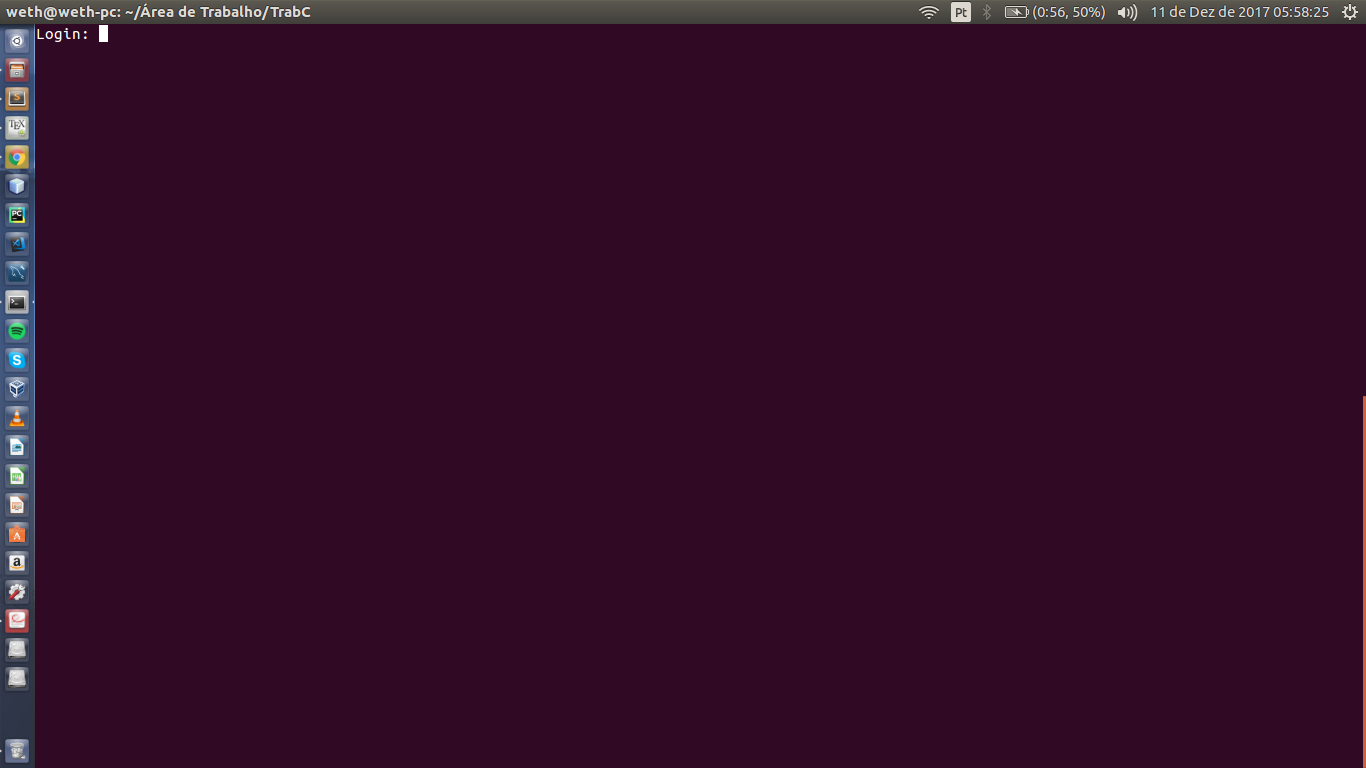
\includegraphics[width=15cm]{img1.png}
\caption{Imagem da Tela de Login}
\label{Rotulo}
\end{figure}
\newpage
Se o login e a senha estiverem corretos, aparecerá uma mensagem assim
\begin{figure}[!htb]
\centering
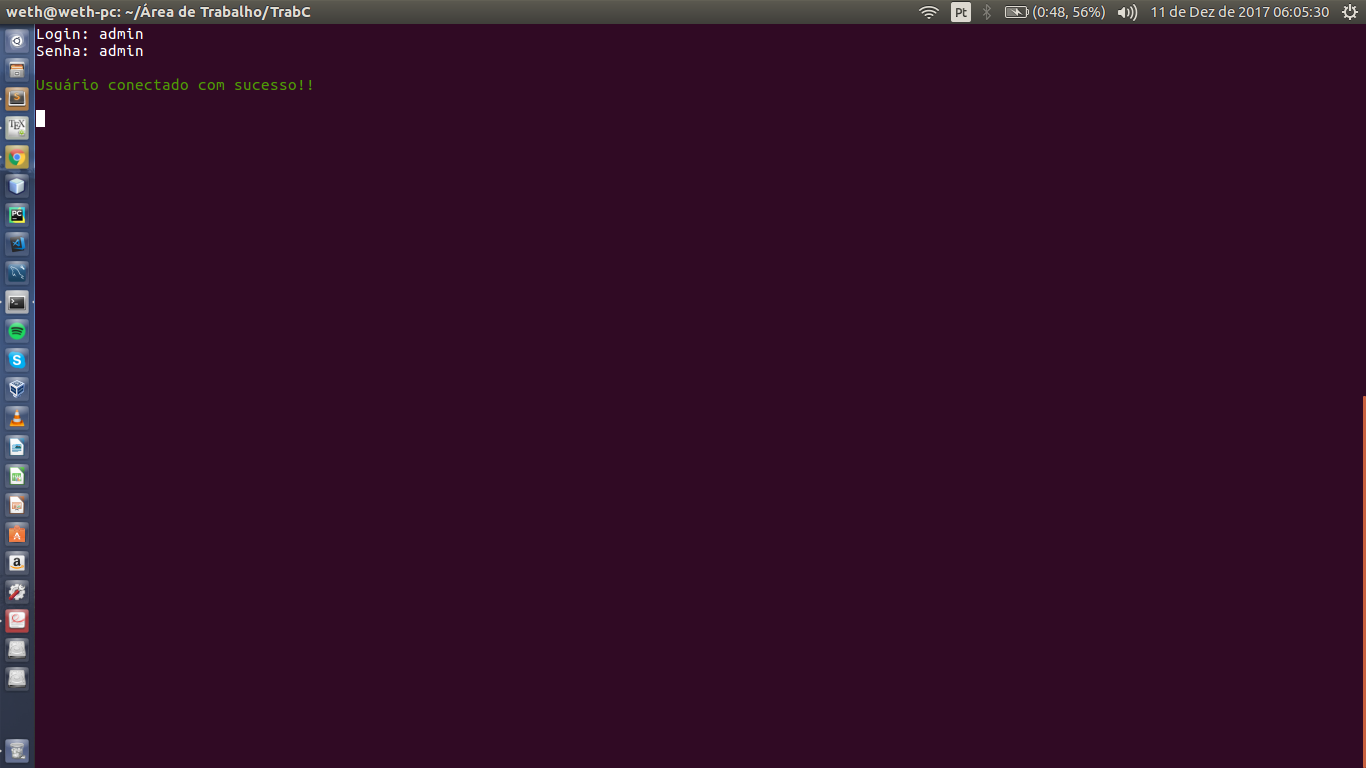
\includegraphics[width=15cm]{img2.png}
\caption{Imagem2 da Tela de Login}
\label{Rotulo}
\end{figure}
\newpage
Outro procedimento seria em digitar um comando, no exemplo será o comando de cadastro de hospedes
\begin{figure}[!htb]
\centering
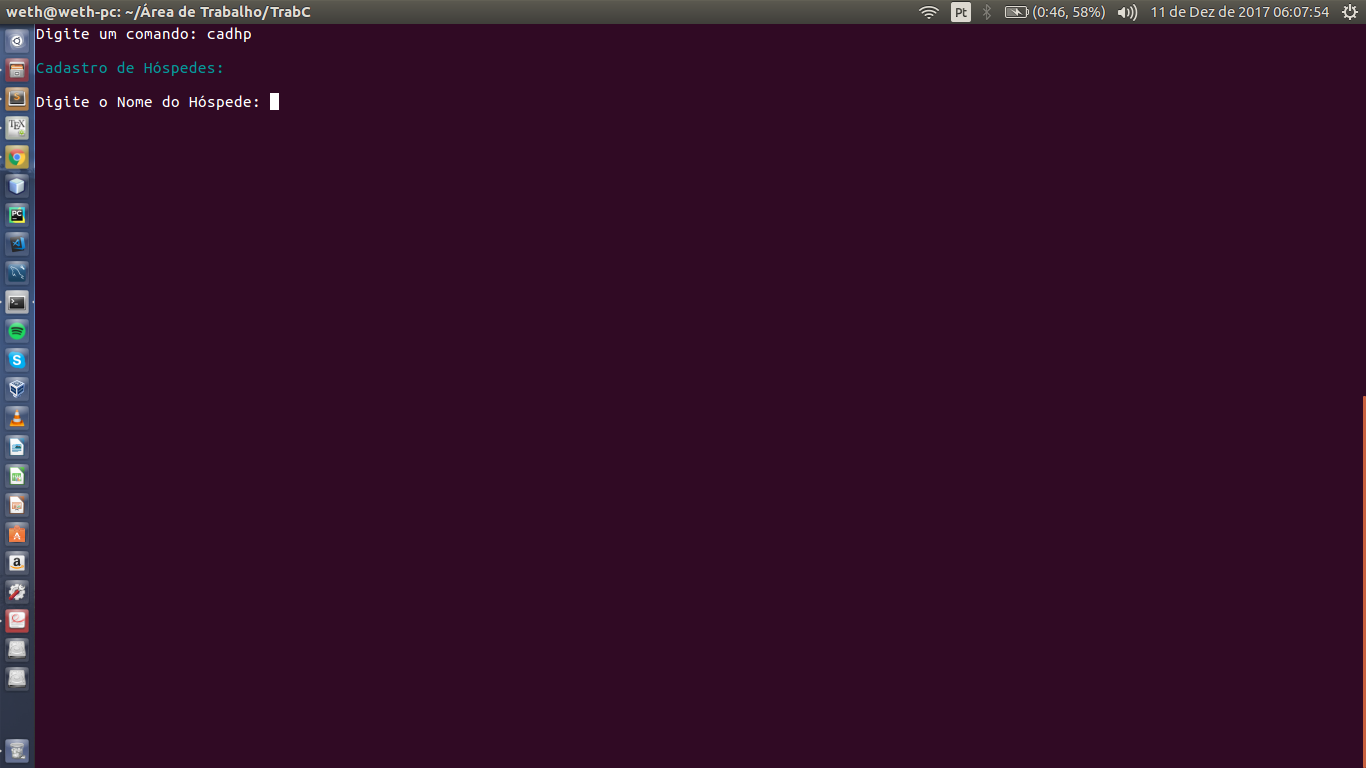
\includegraphics[width=15cm]{img3.png}
\caption{Imagem da Tela do Sistema, onde foi digitado o comando de Cadastro de Hospedes}
\label{Rotulo}
\end{figure}
\newpage
Após serem digitados todos os dados(nesse caso dados hipotéticos), será mostra uma mensagem de sucesso(verde - sucesso, amarelo - atenção, vermelho - perigo/gravidade, azul-claro - legenda.)
\begin{figure}[!htb]
\centering
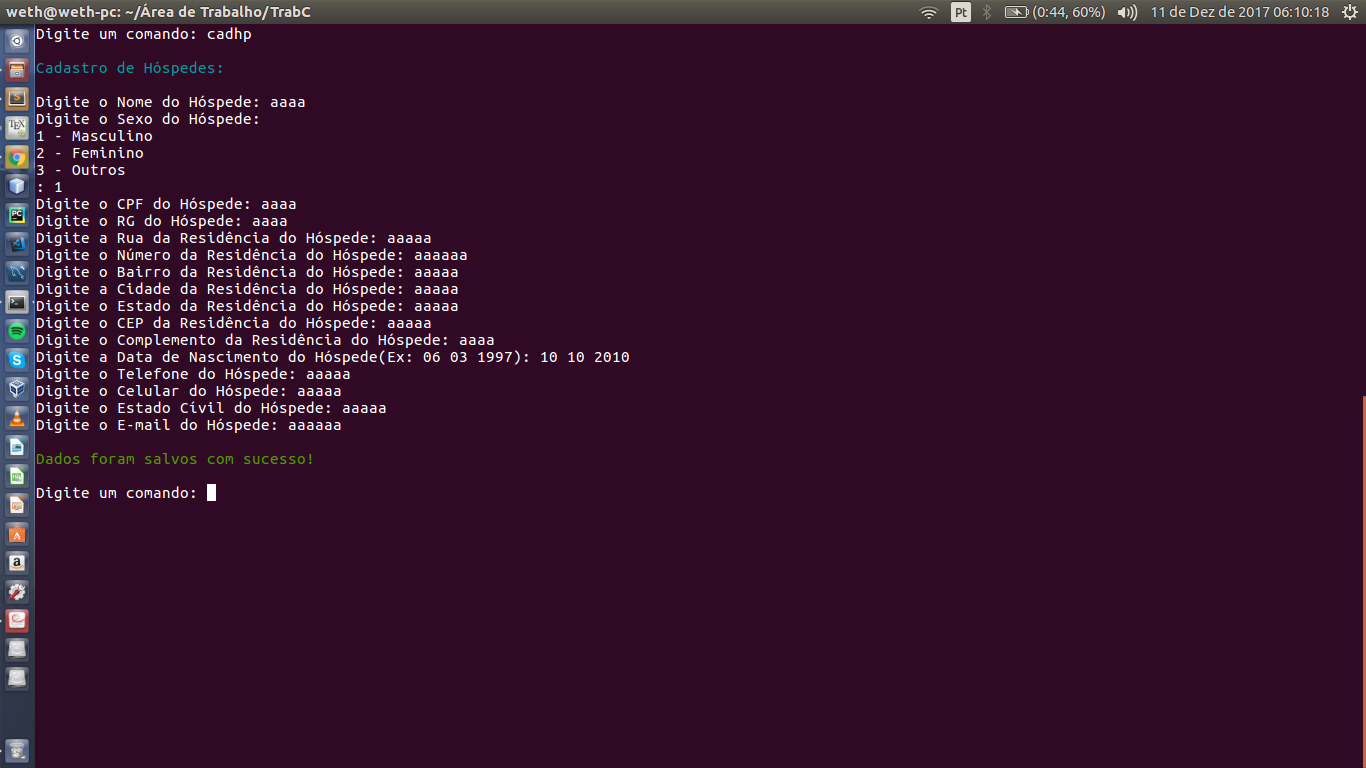
\includegraphics[width=15cm]{img4.png}
\caption{Imagem2 da Tela do Sistema, onde foi digitado o comando de Cadastro de Hospedes}
\label{Rotulo}
\end{figure}
\end{document}	
